In this chapter, we apply the principles of this course to \emph{second} derivatives, which are conceptually just derivatives of derivatives but turn out to have many interesting ramifications.  We begin with a (probably) familiar case of scalar-valued functions from multi-variable calculus, in which the second derivative is simply a matrix called the \emph{Hessian}.  Subsequently, however, we will show that similar principles can be applied to more complicated input and output spaces, generalizing to a notion of $f''$ as a \emph{symmetric bilinear map}.

\subsection{Hessian matrices of scalar-valued functions}
\label{sec:Hessian-scalar}

Recall that for a function $f(x) \in \mathbb{R}$ that maps column vectors $x \in \mathbb{R}^n$ to scalars ($f: \mathbb{R}^n \mapsto \mathbb{R}$), the first derivative $f'$ can be expressed in terms of the familiar gradient $\nabla f = (f')^T$ of multivariable calculus:
$$
\nabla f = \begin{pmatrix} \frac{\partial f}{\partial x_1} \\ \frac{\partial f}{\partial x_2} \\ \vdots \\ \frac{\partial f}{\partial x_n}
\end{pmatrix} \, .
$$
If we think of $\nabla f$ as a new (generally nonlinear) function mapping $x \in \mathbb{R}^n \mapsto \nabla f \in \mathbb{R}^n$, then its derivative is an $n \times n$ Jacobian matrix (a linear operator mapping vectors to vectors), which we can write down explicitly in terms of \emph{second} derivatives of $f$:
$$
  (\nabla f)' =
\begin{pmatrix}
   \frac{\partial^2 f}{ \partial x_1^2} & \cdots & \frac{\partial^2 f}{\partial x_n \partial x_1} \\
        \vdots  &\ddots & \vdots \\
        \frac{\partial^2 f}{\partial x_1 \partial x_n} & \cdots & \frac{\partial^2 f}{\partial x_n \partial x_n}
    \end{pmatrix} = H \, .
$$
This matrix, denoted here by $H$, is known as the \textbf{Hessian} of $f$, which has entries:
\[
H_{i,j} = \frac{\partial^2 f}{ \partial x_j \partial x_i} = \frac{\partial^2 f}{ \partial x_i \partial x_j} = H_{j,i}  \, .
\]
The fact that you can take partial derivatives in either order is a familiar fact from multivariable calculus (sometimes called the ``symmetry of mixed derivatives'' or ``equality of mixed partials''), and means that the Hessian is a \emph{symmetric matrix} $H = H^T$.  (We will later see that such symmetries arise very generally from the construction of second derivatives.)

\begin{example}
For $x \in \mathbb{R}^2$ and the function $f(x) = \sin(x_1) + x_1^2 x_2^3$, its gradient is
$$
\nabla f = \begin{pmatrix} \cos(x_1) + 2x_1 x_2^3 \\
3 x_1^2 x_2^2
\end{pmatrix} \, ,
$$
and its Hessian is
$$
H = (\nabla f)' = \begin{pmatrix} -\sin(x_1) + 2x_2^3 & 6 x_1 x_2^2 \\
6 x_1 x_2^2 & 6 x_1^2 x_2 \end{pmatrix} = H^T \, .
$$
\end{example}

If we think of the Hessian as the Jacobian of $\nabla f$, this tells us that $H \, dx$ predicts the change in $\nabla f$ to first order:
$$
d(\nabla f) = \evalat{\nabla f}{x+dx} - \evalat{\nabla f}{x} = H \, dx \, .
$$
Note that $\evalat{\nabla f}{x+dx}$ means $\nabla f$ evaluated at $x+dx$, which is very different from $df = (\nabla f)^T dx$, where we act $f'(x)=(\nabla f)^T$ \emph{on} $dx$.

Instead of thinking of $H$ of predicting the \emph{first}-order change in $\nabla f$, however, we can also think of it as predicting the \emph{second}-order change in $f$, a \textbf{quadratic approximation} (which could be viewed as the first three terms in a multidimensional Taylor series):
$$
f(x+\delta x) = f(x) + (\nabla f)^T \, \delta x + \frac{1}{2} \delta x^T \, H \, \delta x + o(\Vert \delta x \Vert^2) \, ,
$$
where both $\nabla f$ and $H$ are evaluated at $x$, and we have switched from an infinitesimal $dx$  to a finite change $\delta x$ so that we emphasize the viewpoint of an \emph{approximation} where terms higher than second-order in $\Vert \delta x \Vert$ are dropped.   You can derive this in a variety of ways, e.g. by taking the derivative of both sides with respect to $\delta x$ to reproduce $\evalat{\nabla f}{x+\delta x} = \evalat{\nabla f}{x} + H \, \delta x + o(\delta x)$: a quadratic approximation for $f$ corresponds to a linear approximation for $\nabla f$.   Related to this equation, another useful (and arguably more fundamental) relation that we can derive (and \emph{will} derive much more generally below) is:
$$
dx^T H dx' = f(x + \d x + \d x') + f(x) - f(x + \d x) - f(x + \d x') = f''(x)[dx,dx'] \, 
$$
where $dx$ and $dx'$ are two independent ``infinitesimal'' directions and we have dropped terms of higher than second order.   This formula is very suggestive, because it uses $H$ to map \emph{two} vectors into a \emph{scalar}, which we will generalize below into the idea of a \textbf{bilinear map} $f''(x)[dx,dx']$.  This formula is also obviously symmetric with respect to interchange of $dx$ and $dx'$ --- $f''(x)[dx,dx'] = f''(x)[dx',dx]$ --- which will lead us once again to the symmetry $H=H^T$ below.

\begin{remark}
Consider the Hessian matrix versus other Jacobian matrices.  The Hessian matrix expresses the \emph{second} derivative of a scalar-valued multivariate function, and is always square and symmetric.  A Jacobian matrix, in general, expresses the \emph{first} derivative of a vector-valued multivariate function, may be non-square, and is rarely symmetric.  (However, the Hessian matrix \emph{is} the Jacobian of the $\nabla f$ function!)
\end{remark}

\subsection{General second derivatives: Bilinear maps}

Recall, as we have been doing throughout this class, that we define the derivative of a function $f$ by a linearization of its change $\d f$ for a small (``infinitesimal'') change $\d x$ in the input: 
\[
\d f = f(x + \d x) - f(x) = f'(x) [\d x] \, ,
\]
implicitly dropping higher-order terms.
If we similarly consider the second derivative $f''$ as simply the same process applied to $f'$ instead of $f$, we  obtain the following formula, which is easy to write down but will take some thought to interpret: 
\[
d f' = f'(x + \d x') - f'(x) = f''(x) [\d x'].
\]
(Notation: $\d x'$ is not some kind of derivative of $\d x$; the prime simply denotes a \emph{different}
arbitrary small change in~$x$.) What kind of ``thing'' is $df'$?   Let's consider a simple concrete example:

\begin{example}
Consider the following function $f(x): \mathbb{R}^2 \mapsto \mathbb{R}^2$ mapping two-component vectors $x \in \mathbb{R}^2 $ to two-component vectors $f(x) \in \mathbb{R}^2$:
$$
f(x) = \begin{pmatrix} x_1^2 \sin(x_2) \\ 5x_1 - x_2^3
\end{pmatrix} \, .
$$
Its first derivative is described by a $2\times 2$ Jacobian matrix:
$$
f'(x) = \begin{pmatrix}
2x_1 \sin(x_2) & x_1^2 \cos(x_2) \\
5 & -3x_2^2
\end{pmatrix}
$$
that maps a small change $dx$ in the input vector $x$ to the corresponding small change $df = f'(x)dx$ in the output vector $f$.

What is $df' = f''(x)[dx']$?  It must take a small change $dx' = (dx_1', dx_2')$ in $x$ and return the first-order change $df' = f'(x+dx')-f'(x)$ in our Jacobian matrix $f'$.  If we simply take the differential of each entry of our Jacobian (a function from vectors $x$ to matrices $f'$), we find:
$$
df' = 
\begin{pmatrix}
2\,dx_1' \sin(x_2) + 2x_1 \cos(x_2) \,dx_2' & 2 x_1 \, dx_1' \cos(x_2) - x_1^2 \sin(x_2)\, dx_2' \\
0 & -6x_2\,dx_2'
\end{pmatrix}
= f''(x)[dx']
$$
That is, $df'$ is a $2\times 2$ matrix of ``infinitesimal'' entries, of the same shape as $f'$.

From this viewpoint, $f''(x)$ is a linear operator acting on vectors $dx'$ and outputting $2\times 2$ matrices $f''(x)[dx']$, but this is one of the many cases where it is easier to write down the linear operator as a ``rule'' than as a ``thing'' like a matrix.  The ``thing'' would have to either be some kind of ``three-dimensional matrix'' or we would have to ``vectorize'' $f'$ into a ``column vector'' of 4 entries in order to write its $4\times 4$ Jacobian, as in Sec.~\ref{sec:kronecker} (which can obscure the underlying structure of the problem).

Furthermore, since this $df'$ is a linear operator (a matrix), we can act it on \emph{another} vector $dx = (dx_1, dx_2)$ to obtain:
$$
df' \begin{pmatrix} dx_1 \\ dx_2 \end{pmatrix} =
\begin{pmatrix}
2 \sin(x_2) \,dx_1'\,dx_1 + 2x_1 \cos(x_2) (\,dx_2'\,dx_1 + \, dx_1' \, dx_2) - x_1^2 \sin(x_2)\, dx_2' \, dx_2 \\
-6x_2\,dx_2' \,dx_2
\end{pmatrix} = f''(x)[dx'][dx] \, .
$$
Notice that \emph{this} result, which we will call $f''(x)[dx', dx]$ below, is the ``same shape'' as $f(x)$ (a 2-component vector).  Moreover, it doesn't change if we swap $dx$ and $dx'$: $f''(x)[dx', dx] = f''(x)[dx, dx']$, a key symmetry of the second derivative that we will discuss further below.
\end{example} 

$df'$ is an (infinitesimal) object of the same ``shape'' as $f'(x)$, \emph{not} $f(x)$.  Here, $f'$ is a linear operator,
so its change $\d f'$ must \emph{also} be an (infinitesimal) linear operator (a ``small change'' in a linear operator)
that we can therefore act on an arbitrary
$\d x$ (or $\delta x$), in the form: 
\[
df'[dx] = f''(x) [\d x'][\d x] := f''(x) [\d x', \d x] \, ,
\]
where we combine the two brackets for brevity. This final result $f''(x) [\d x', \d x]$ is the same type of object (vector) as the original output $f(x)$.  This implies that $f''(x)$ is a \textit{bilinear map}: acting on \textbf{two} vectors, and linear in either vector taken individually.  (We will see shortly that the ordering of $dx$ and $dx'$ doesn't matter: $f''(x)[dx',dx]=f''(x)[dx,dx']$.)  

More precisely, we have the following.
\begin{definition}[Bilinear Map]
    Let $U,V,W$ be a vector spaces, not necessarily the same. Then, a \textbf{bilinear map} is a function $B:U\times V \to W$, mapping a $u \in U$ and $v \in V$ to $B[u,v] \in W$, such that we have linearity in both arguments:
    \[
    \begin{cases}
        B[u, \alpha v_1 + \beta v_2] = \alpha B[u,v_1] + \beta B[u,v_2] \\
        B[\alpha u_1 + \beta u_2, v] = \alpha B[u_1,v] + \beta B[u_2,v]
    \end{cases}
    \]
     for any scalars $\alpha, \beta$,

     If $W = \mathbb{R}$, i.e.~the output is a scalar, then it is called a \textbf{bilinear form}.
\end{definition}

Note that in general, even if $U = V$ (the two inputs $u,v$ are the ``same type'' of vector) we may have $B[u,v] \neq B[v,u]$, but in the case of $f''$ we have something very special that happens. In particular, we can show that $f''(x)$ is a \textit{symmetric bilinear map}, meaning 
\[
f''(x) [\d x', \d x] = f''(x) [\d x, \d x']
\]
for any $\d x$ and $\d x'$.  Why? Because, applying the definition of $f''$ as giving the change in $f'$ from $\d x'$, and then the definition of $f'$ as giving the change in $f$ from $\d x$, we can  re-order terms to obtain: 
\begin{align*}
    f''(x) [\d x', \d x] &= f'(x + 
    \d x') [\d x] - f'(x) [\d x] \\
    &= \left(f(x+ \underbrace{\d x' + \d x}_{= \d x + \d x'}) - f(x+ \d x')\right) - \left(f(x+ \d x) - f(x)\right) \\ 
    &= \boxed{f(x + \d x + \d x') + f(x) - f(x + \d x) - f(x + \d x')} \\
    &= \left(f(x + \d x + \d x')  - f(x + \d x)\right) - \left(f(x + \d x') - f(x)\right) \\
    &= f'(x + 
    \d x) [\d x'] - f'(x) [\d x'] \\
    &= f''(x) [\d x, \d x'] \, 
\end{align*}
where we've boxed the middle formula for $f''$ which emphasizes its symmetry in a natural way.
(The basic reason why this works is that the ``$+$'' operation is always \emph{commutative} for any vector space. A geometric interpretation is depicted in Fig.~\ref{fig:second-deriv}.)

\begin{figure}
\begin{center}
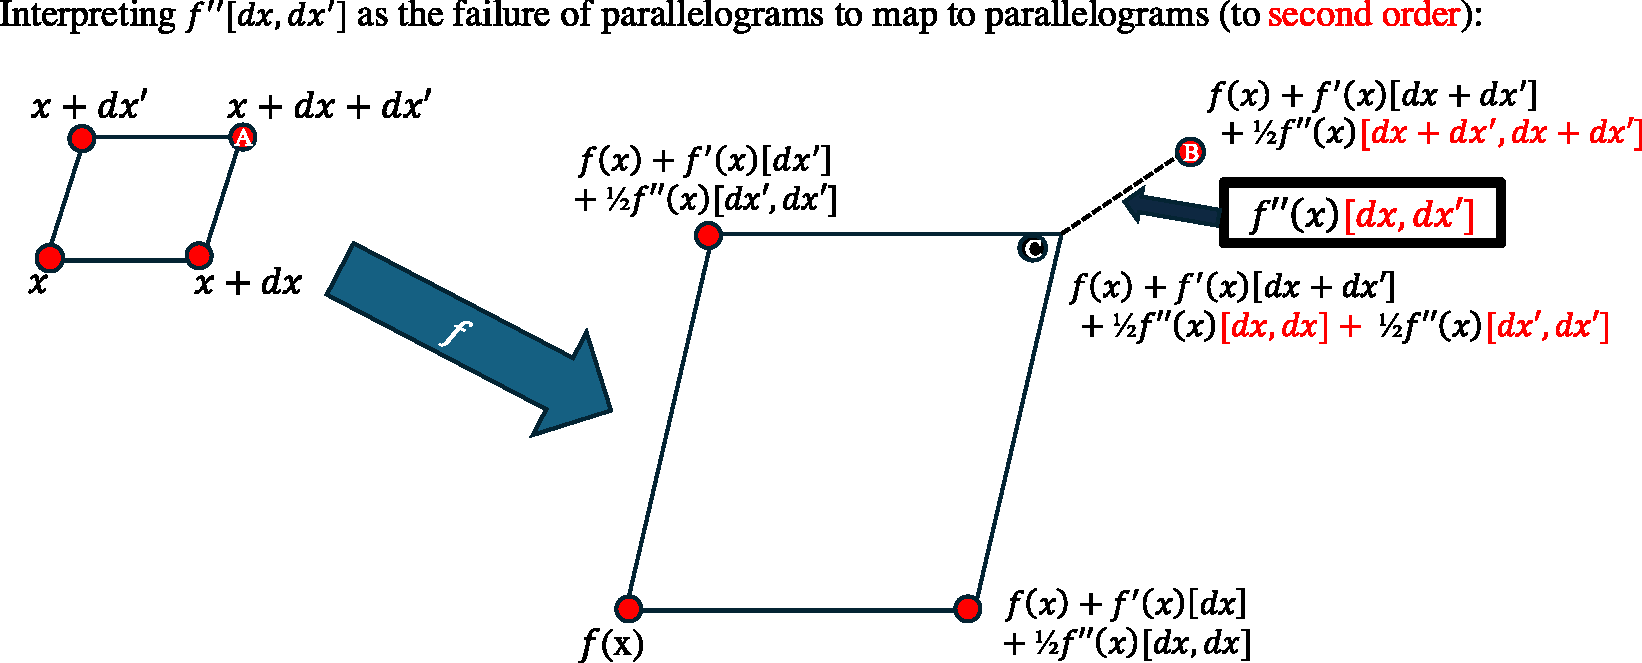
\includegraphics[width=0.8\textwidth]{figures/second-derivative.pdf}
\end{center}
\caption{Geometric interpretation of $f''(x)[dx,dx']$:
To first order, a function $f$ maps parallelograms to parallelograms.  To second order, however it ``opens'' parallelograms: The deviation from point $B$ (the image of $A$) from point $C$ (the completion of the parallelogram) is the second
derivative $f''(x)[dx,dx']$.  
The symmetry of $f''$ as a bilinear form can be traced back  geometrically 
to the mirror symmetry of the input parallelogram across its diagonal
from $x$ to point~A. \label{fig:second-deriv}
}
\end{figure}

\begin{example}
    Let's review the familiar example from multivariable calculus, $f: \R^n \to \R$. That is, $f(x)$ is a scalar-valued function of a column vector $x\in \R^n$.  What is $f''$?
\end{example}
Recall that 
\[
f'(x) = (\nabla f)^T \implies f'(x) [\d x] = \text{scalar } \d f = (\nabla f)^T \d x. 
\]
Similarly, 
\begin{align*}
    f''(x) [\d x', \d x] &= \text{scalar from two vectors, linear in both} \\
    &= \d x'^T H \d x \, ,
\end{align*}
where $H$ must be exactly the $n \times n$ matrix  \textbf{Hessian matrix} introduced in Sec.~\ref{sec:Hessian-scalar}, since an expression like $\d x'^T H \d x$ is the most general possible bilinear form mapping two vectors to a scalar.  Moreover, since we now know that $f''$ is always a \emph{symmetric} bilinear form, we must have:
\begin{align*}
f''(x) [\d x', \d x] &=\d x'^T H \d x \\
&= f''(x) [\d x, \d x'] = \d x^T H \d x' =
     (\d x^T H \d x')^T  \qquad (\mathrm{scalar} = \mathrm{scalar}^T)\\
    &= \d x'^T H^T \d x 
\end{align*}
for all $dx$ and $dx'$.
This implies that $H = H^T$: the Hessian matrix is symmetric.  As discussed in Sec.~\ref{sec:Hessian-scalar}, we already knew this from multi-variable calculus.  Now, however, this ``equality of mixed partial derivatives'' is simply a special case of $f''$ being a symmetric bilinear map.

As an example, let's consider a special case of the general formula above:

\begin{example}
    Let $f(x) = x^T A x$ for $x \in \R^n$ and $A$ an $n \times n$ matrix. As above, $f(x) \in \R$ (scalar outputs). Compute $f''$.
\end{example}

The computation is fairly straightforward. Firstly, we have that 
\[
f' = (\nabla f)^T = x^T(A + A^T).
\]
This implies that $\nabla f = (A + A^T) x$, a linear function of $x$. Hence, the Jacobian of $\nabla f$ is the Hessian
$f'' = H = A + A^T$. Furthermore, note that this implies 
\begin{align*}
    f(x) &= x^T A x = (x^T A x)^T  \qquad (\mathrm{scalar} = \mathrm{scalar}^T)\\
    &= x^T A^T x \\
    &= \frac{1}{2} (x^T A x + x^T A^T x) = \frac{1}{2} x^T (A + A^T) x\\
    &= \frac{1}{2} x^T H x = \frac{1}{2} f''[x,x] \, ,
\end{align*}
which will turn out to be a special case of the quadratic approximations of Sec.~\ref{sec:Hessian-quadratic} (exact in this example since $f(x)=x^T A x$ is quadratic to start with).

\begin{example}
    Let $f(A) = \det A$ for $A$ an $n\times n$ matrix. Express $f''(A)$ as a rule for $f''(A)[dA,dA']$ in terms of $\d A$ and $\d A'$.
\end{example}

From lecture 3, we have the first derivative 
\[
f'(A) [\d A] = \d f = \det (A) \tr(A^{-1} \d A).
\]
Now, we want to compute the change $d'(df) = d'(f'(A)[dA]) = f'(A+dA')[dA] - f'(A)[dA]$ in this formula, i.e.~the differential (denoted $d'$) where we change $A$ by $dA'$ while treating $dA$ as a constant:
\begin{align*}
    f''(A) [\d A, \d A'] &= \d ' (\det A \tr (A^{-1} \d A)) \\
    &= \det A \tr(A^{-1} \d A') \tr(A^{-1} \d A) - \det A \tr(A^{-1} \,\d A' A^{-1}\, \d A) \\
    &= f''(A) [\d A', \d A]
\end{align*}
where the last line (symmetry) can be derived
explicitly by the cyclic property of the trace (although of course it must be true for any $f''$).  Although $f''$ here is a perfectly good bilinear form acting on matrices $dA,dA'$, it is not very natural to express $f''$ as a ``Hessian matrix.''

If we really wanted to express $f''$ in terms of an explicit Hessian matrix, we could use the the ``vectorization'' approach of Sec.~\ref{sec:kronecker}.
Let us consider, for example, the term $\tr(A^{-1} \,\d A' A^{-1}\, \d A)$ using Kronecker products (Sec.~\ref{sec:kronecker}).  In general, for matrices $X,Y,B,C$:
$$
(\vecm{X})^T (B \otimes C) \vecm{Y} = (\vecm{X})^T \vecm{(CYB^T)} = \tr(X^T CYB^T) = \tr(B^T X^T CY) \, ,
$$
recalling that $(\vecm{X})^T \vecm{Y} = \tr(X^T Y)$ is the Frobenius inner product (Sec.~\ref{sec:generalvectorspaces}).  Thus,
$$
\tr(A^{-1} \,\d A' A^{-1}\, \d A)
= \vecm{(\d A'^T)}^T (A^{-T} \otimes A^{-1}) \vecm{(\d A)} \, .
$$
This is still not quite in the form we want for a Hessian matrix, however, because it involves $\vecm{(\d A'^T)}$ rather than $\vecm{(\d A')}$ (the two vectors are related by a permutation matrix, sometimes called a ``commutation'' matrix). Completing this calculation would be a nice exercise in mastery of Kronecker products, but getting an explicit Hessian seems like a lot of algebra for a result of dubious utility!

\subsection{Generalized quadratic approximation}
\label{sec:Hessian-quadratic}

So how do we ultimately think about $f''$? We know that $f'$ is the linearization/linear approximation of $f(x)$, i.e. 
\[
f(x + \delta x ) = f(x) + f'(x) [\delta x] + o(\lVert \delta x\rVert).
\] 
Now, just as we did for the simple case of Hessian matrices in Sec.~\ref{sec:Hessian-scalar} above, we can use $f''$ to form a \textit{quadratic approximation} of $f(x)$. In particular, one can show that 
\[
f(x+ \delta x) = f(x) + f'(x) [\delta x] + \frac{1}{2} f''(x) [\delta x, \delta x] +  o (\lVert \delta x\rVert^2).
\]
Note that the $\frac{1}{2}$ factor is just as in the Taylor series. To derive this, simply plug the quadratic approximation into 
\[
f''(x) [\d x, \d x'] = f(x + \d x + \d x') + f(x) - f(x + \d x) - f(x + \d x').
\]
and check that the right-hand side reproduces $f''(x)$.   (Note how $dx$ and $dx'$ appear symmetrically in this formula, which reflects the symmetry of $f''$.)


\subsection{Hessians and optimization}

Many important applications of second derivatives, Hessians, and quadratic approximations arise in optimization: minimization (or maximization) of functions $f(x)$.\footnote{Much of machine learning uses only variations on gradient descent, without incorporating Hessian information except implicitly via ``momentum'' terms.  Partly this can be explained by the fact that optimization problems in ML are typically solved only to low accuracy, often have nonsmooth/stochastic aspects, rarely involve nonlinear constraints, and are often very high-dimensional.  This is only a small corner of the wider universe of computational optimization!}

\subsubsection{Newton-like methods}

When searching for a local minimum (or maximum) of a complicated function $f(x)$, a common procedure is to approximate $f(x+\delta x)$ by a simpler ``model'' function for small $\delta x$, and then to optimize this model to obtain a potential optimization step.   For example, approximating $f(x+\delta x) \approx f(x)+f'(x)[\delta x]$ (an affine model, colloquially called ``linear'') leads to gradient descent and related algorithms.  A better approximation for $f(x + \delta x)$ will often lead to faster-converging algorithms, and so a natural idea is to exploit the \emph{second} derivative $f''$ to make a quadratic model, as above, and accelerate optimization.

For unconstrained optimization, minimizing $f(x)$ corresponds to finding a root of the derivative $f' = 0$ (i.e., $\nabla f = 0$), and a \emph{quadratic} approximation for $f$ yields a first-order (affine) approximation $f'(x + \delta x) \approx f'(x) + f''(x)[\delta x]$ for the derivative $f'$. In $\mathbb{R}^n$, this is $\delta(\nabla f) \approx H \delta x$.  So, minimizing a quadratic model is effectively a \emph{Newton step} $\delta x \approx -H^{-1} \nabla f$ to find a root of $\nabla f$ via first-order approximation.   Thus, optimization via quadratic approximations is often viewed as a form of Newton algorithm.  As discussed below, it is also common to employ \emph{approximate} Hessians in optimization, resulting in ``quasi-Newton'' algorithms.

More complicated versions of this idea arise in optimization with constraints, e.g.~minimizing an objective function $f(x)$ subject to one or more nonlinear inequality constraints $c_k(x) \le 0$.   In such cases, there are a variety of methods that take both first and second derivatives into account, such as ``sequential quadratic programming''\footnote{The term ``programming'' in optimization theory does not refer to software engineering, but is rather an anachronistic term for optimization problems.  For example, ``linear programming'' (LP) refers to optimizing affine objectives and affine constraints, while ``quadratic programming'' (QP) refers to optimizing convex quadratic objectives with affine constraints.} (SQP) algorithms that solve a sequence of ``QP'' approximations involving quadratic objectives with affine constraints (see e.g.~the book \textit{Numerical Optimization} by Nocedal and Wright, 2006).

There are many technical details, beyond the scope of this course, that must be resolved in order to translate such high-level ideas into practical algorithms.
For example, a quadratic model is only valid for small enough $\delta x$, so there must be some mechanism to limit the step size. One possibility is ``backtracking line search'': take a Newton step $x+\delta x$ and, if needed, progressively ``backtrack'' to $x+\delta x/10, x+\delta x/100, \ldots$ until a  sufficiently decreased value of the objective is found.  Another commonplace idea is a ``trust region'': optimize the model with the constraint that $\delta x$ is sufficiently small, e.g.~$\Vert \delta x \Vert \le s$ (a spherical trust region), along with some rules to adaptively enlarge or shrink the trust-region size ($s$) depending on how well the model predicts $\delta f$.  There are many variants of Newton/SQP-like algorithms depending on the choices made for these and other details.

\subsubsection{Computing Hessians}

In general, finding $f''$ or the Hessian is often computationally expensive in higher dimensions. If $f(x): \R^n\to\R$, then the Hessian, $H$, is an $n\times n$ matrix, which can be huge if $n$ is large---even storing $H$ may be prohibitive, much less computing it. When using automatic differentiation (AD), Hessians are often computed by a \emph{combination} of forward and reverse modes (Sec.~\ref{sec:forward-over-reverse}), but AD does not circumvent the fundamental scaling difficulty for large~$n$.

Instead of computing $H$ explicitly, however, one can instead \emph{approximate} the Hessian in various ways; in the context of optimization, approximate Hessians are found in ``quasi-Newton'' methods such as the famous ``BFGS'' algorithm and its variants. One can also derive efficient methods to compute Hessian--vector products $Hv$ without computing $H$ explicitly, e.g.~for use in Newton--Krylov methods.   (Such a product $Hv$ is equivalent to a directional derivative of $f'$, which is efficiently computed by ``forward-over-reverse'' AD as in Sec.~\ref{sec:forward-over-reverse}.)

\subsubsection{Minima, maxima, and saddle points}

Generalizing the rules you may recall from single- and multi-variable calculus, we can use the second derivative to determine whether an extremum is a minimum, maximum, or saddle point. Firstly, an extremum of a scalar function $f$ is a point $x_0$  such that $f'(x_0) = 0$. That is, 
\[
f'(x_0) [\delta x] = 0
\] 
for \textit{any} $\delta x$. Equivalently, 
\[
\nabla f \bigr|_{x_0} = f'(x_0)^T = 0.
\]

Using our quadratic approximation around $x_0$, we then have that 
\[
f(x_0 + \delta x) = f(x_0) + \underbrace{f'(x_0) [\delta x]}_{=0} + \frac{1}{2} f''(x_0) [\delta x, \delta x] + o(\lVert \delta x\rVert^2).
\]
The definition of a local minimum $x_0$ is that $f(x_0 + \delta x ) > f(x_0)$ for any $\delta x \neq 0$ with $\lVert \delta x\rVert$ sufficiently small. To achieve this at a point where $f' = 0$, it is enough to have $f''$ be a positive-definite quadratic form:
\[
f''(x_0) [\delta x, \delta x] >0 \text{ for all } \delta x \ne 0 \iff \textbf{positive-definite } f''(x_0) \, .
\]

For example, for inputs $x\in \R^n$, so that $f''$ is a real-symmetric $n \times n$ Hessian matrix, $f''(x_0) = H(x_0) = H(x_0)^T$, this corresponds to the usual criteria for a positive-definite matrix: 
\[
f''(x_0) [\delta x, \delta x] = \delta x^T H(x_0) \delta x >0 \text{ for all } \delta x \ne 0 \iff H(x_0) \text{ positive-definite } \iff \text{all eigenvalues of } H(x_0) > 0.
\]

In first-year calculus, one often focuses in particular on the 2-dimensional case, where $H$ is a $2\times 2$ matrix.  In the $2\times 2$ case, there is a simple way to check the signs of the two eigenvalues of $H$, in order to check whether an extremum is a minimum or maximum: the eigenvalues are both positive if and only if $\det (H) >0$ and $\tr(H)  >0$, since $\det (H) = \lambda_1 \lambda_2$ and $\tr(H) = \lambda_1 + \lambda_2$. In higher dimensions, however, one needs more complicated techniques to compute eigenvalues and/or check positive-definiteness, e.g.~as discussed in MIT courses 18.06 (Linear Algebra) and/or 18.335 (Introduction to Numerical Methods).  (In practice, one typically checks positive-definiteness by performing a form of Gaussian elimination, called a Cholesky factorization, and checking that the diagonal ``pivot'' elements are $> 0$, rather than by computing eigenvalues which are much more expensive.)

Similarly, a point $x_0$ where $\nabla f = 0$ is a local \emph{maximum}
 if $f''$ is negative-definite, or equivalently if the eigenvalues of the Hessian are all negative. Additionally, $x_0$ is a \emph{saddle} point if $f''$ is indefinite, i.e. the eigenvalues include both positive and negative values. However, cases where some eigenvalues are zero are more complicated to analyze; e.g.~if the eigenvalues are all $\ge 0$ but some are $=0$, then whether the point is a minimum depends upon higher derivatives.

\subsection{Further Reading}

All of this formalism about ``bilinear forms'' and so forth may seem like a foray into abstraction for the sake of abstraction.  Can't we always reduce things to ordinary matrices by choosing a basis (``vectorizing'' our inputs and outputs)?  However, we often don't \emph{want} to do this for the same reason that we often prefer to express first derivatives as linear operators rather than as explicit Jacobian matrices.   Writing linear or bilinear operators as explicit matrices, e.g.~$\vecm(A\,dA + dA\,A) = (I\otimes A + A^T \otimes I)\vecm(dA)$ as in Sec.~\ref{sec:kronecker}, often disguises the underlying structure of the operator and introduces a lot of algebraic complexity for no purpose, as well as being potentially computationally costly (e.g.~exchanging small matrices $A$ for large ones $I \otimes A$). 

As we discussed in this chapter, an important generalization of quadratic operations to arbitrary vector spaces come in the form of \href{https://en.wikipedia.org/wiki/Bilinear_map}{bilinear maps} and \href{https://en.wikipedia.org/wiki/Bilinear_form}{bilinear forms}, and there are many textbooks and other sources discussing these ideas and variations thereof. For example, we saw that the second derivative can be seen as a \href{https://en.wikipedia.org/wiki/Symmetric_bilinear_form}{symmetric bilinear form}. This is closely related to a \href{https://en.wikipedia.org/wiki/Quadratic_form}{quadratic form} $Q[x]$, which what we get by plugging the same vector twice into a symmetric bilinear form $B[x,y]=B[y,x]$, i.e.~$Q[x] = B[x,x]$.  (At first glance, it may seem like $Q$ carries ``less information'' than $B$, but in fact this is not the case.  It is easy to see that one can recover $B$ from $Q$ via $B[x,y] = (Q[x+y] - Q[x-y])/4$, called a ``polarization identity.'') For example, the $f''(x) [\delta x, \delta x]/2$ term that appears in quadratic approximations of $f(x+ \delta x)$ is a quadratic form. The most familiar multivariate version of $f''(x)$ is the \href{https://en.wikipedia.org/wiki/Hessian_matrix}{Hessian matrix} when $x$ is a column vector and $f(x)$ is a scalar, and Khan Academy has an elementary \href{https://www.khanacademy.org/math/multivariable-calculus/applications-of-multivariable-derivatives/quadratic-approximations/a/quadratic-approximation}{introduction to quadratic approximation}.

\href{https://en.wikipedia.org/wiki/Definite_matrix}{Positive-definite} Hessian matrices, or more generally \href{https://en.wikipedia.org/wiki/Definite_quadratic_form}{definite quadratic forms} $f''$, appear at extrema ($f' =0$) of scalar-valued functions $f(x)$ that are local minima. There are a lot \href{http://www.columbia.edu/~md3405/Unconstrained_Optimization.pdf}{more formal treatments} of the same idea, and conversely Khan Academy has the \href{https://www.khanacademy.org/math/multivariable-calculus/applications-of-multivariable-derivatives/optimizing-multivariable-functions/a/second-partial-derivative-test}{simple 2-variable version} where you can check the sign of the $2\times 2$ eignevalues just by looking at the determinant and a single entry (or the trace). There's a nice \href{https://math.stackexchange.com/questions/2285282/relating-condition-number-of-hessian-to-the-rate-of-convergence}{stackexchange discussion} on why an \href{https://nhigham.com/2020/03/19/what-is-a-condition-number/}{ill-conditioned} Hessian tends to make steepest descent converge slowly. Some Toronto \href{https://www.cs.toronto.edu/~rgrosse/courses/csc421_2019/slides/lec07.pdf}{course notes on the topic} may also be useful.

Lastly, see for example these Stanford notes on \href{https://web.stanford.edu/class/ee364b/lectures/seq_notes.pdf}{sequential quadratic optimization} using trust regions (Section 2.2), as well as the 18.335 \href{https://github.com/mitmath/18335/blob/spring21/notes/BFGS.pdf}{notes on BFGS quasi-Newton methods}. The fact that a quadratic optimization problem in a sphere has \href{https://en.wikipedia.org/wiki/Strong_duality}{strong duality}, and hence is efficiently solvable, is discussed in Section 5.2.4 of the \href{https://web.stanford.edu/~boyd/cvxbook/}{\textit{Convex Optimization} book}. There has been a lot of work on \href{https://en.wikipedia.org/wiki/Hessian_automatic_differentiation}{automatic Hessian computation}, but for large-scale problems you may only be able to compute Hessian--vector products efficiently in general, which are equivalent to a directional derivative of the gradient and can be used (for example) for \href{https://en.wikipedia.org/wiki/Newton%E2%80%93Krylov_method}{Newton--Krylov methods}.

The Hessian matrix is also known as the ``curvature matrix"
especially in optimization. If we have a scalar function $f(x)$ of $n$ variables, its ``graph'' is the set of points $(x,f(x))$ in $R^{n+1}$; we call the last dimension the ``vertical" dimension. At a ``critical point'' $x$ (where $\nabla f = 0$), then $v^T H v$  is the ordinary curvature sometimes taught in first-year calculus, of the curve obtained by intersecting the graph with the plane in the direction $v$ from $x$ and the vertical (the ``normal section''). The determinant of $H$, sometimes known as the Hessian determinant, yields the Gaussian curvature.

A closely related idea is the derivative of the unit normal.  For a graph as in the 
preceding paragraph we may assume that $f(x)=x^THx/2$ to second order.  It is easy
to see that at any point $x$ the tangents have the form $(dx, f'(x)[dx])=(dx,x^THdx)$
and the normal is then $(Hx,1)$.  Near $x=0$ this a unit normal to second order, and
its derivative is $(Hdx,0)$.  Projecting onto the horizontal, we see that the Hessian
is the derivative of the unit normal.  This is called the ``shape operator" in differential
geometry.


\todo{ The Hessian matrix is also known as the ``curvature matrix"
especially in the fields of optimization.
If we have a scalar function $f(x)$ of $n$ variables the graph of a function is the set of points $(x,f(x))$ in $R^{n+1}$. 
We call the last dimension the ``vertical" dimension.
At a critical point $x$ (meaning 0 gradient), we have $v^THv$ 
is the ordinary curvature taught in some calculus classes of the curve obtained by intersecting the graph with the plane in the direction $v$ from $x$ and the vertical.  (The ``normal section").
The determinant, sometimes known as the Hessian determinant,
is the Gaussian curvature (up to sign because of the embedding??).
Alternatively, one can take a tangent plane to be the horizontal
(effectively rotating the graph) and then the Hessian has
the same properties as above at any point.
Yet another equivalent way to say this, perhaps a bit more elegantly,
is to consider the magnitude of the derivative of the unit normal
with resepect to tangents.  (The derivative
is a function from tangents to tangents.)
TODO: Confirm that the scalar curvature is the sum of the eigenvalues taken two at a time, and write down the Riemannian and Ricci curvature, and place in another chapter?  I think the Ricci curvature is related
to sums of two by two determinants of the Hessian, in other words, it is related to the second compound matrix of the Hessian.
Also in some other chapter some day, maybe go so far as talking
about ...?}
